\documentclass{standalone}
\usepackage{tikz}
\usetikzlibrary{patterns, positioning}


\begin{document}
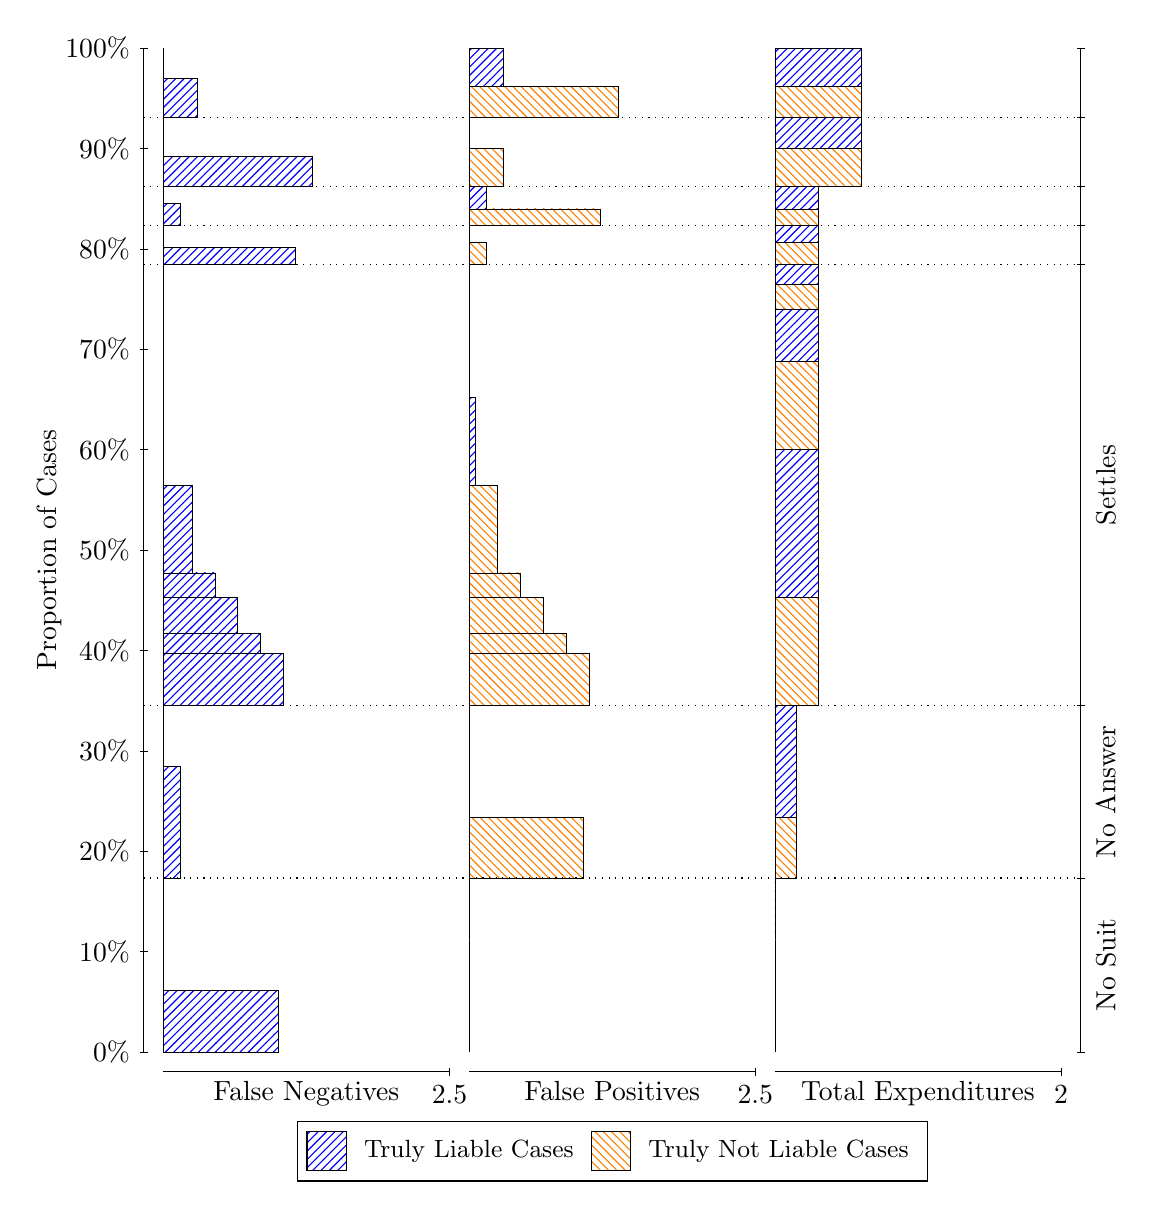
\begin{tikzpicture}
\draw[black, very thin] (1.5,1.75) -- (1.5,14.5);
\node[rotate=90, text=black, anchor=center] at (0.3, 8.125) {Proportion of Cases};
\draw[black, very thin] (1.45,1.75) -- (1.55,1.75);
\node[text=black, anchor=east] at (1.45, 1.75) {0\%};
\draw[black, very thin] (1.45,3.025) -- (1.55,3.025);
\node[text=black, anchor=east] at (1.45, 3.025) {10\%};
\draw[black, very thin] (1.45,4.3) -- (1.55,4.3);
\node[text=black, anchor=east] at (1.45, 4.3) {20\%};
\draw[black, very thin] (1.45,5.575) -- (1.55,5.575);
\node[text=black, anchor=east] at (1.45, 5.575) {30\%};
\draw[black, very thin] (1.45,6.85) -- (1.55,6.85);
\node[text=black, anchor=east] at (1.45, 6.85) {40\%};
\draw[black, very thin] (1.45,8.125) -- (1.55,8.125);
\node[text=black, anchor=east] at (1.45, 8.125) {50\%};
\draw[black, very thin] (1.45,9.4) -- (1.55,9.4);
\node[text=black, anchor=east] at (1.45, 9.4) {60\%};
\draw[black, very thin] (1.45,10.675) -- (1.55,10.675);
\node[text=black, anchor=east] at (1.45, 10.675) {70\%};
\draw[black, very thin] (1.45,11.95) -- (1.55,11.95);
\node[text=black, anchor=east] at (1.45, 11.95) {80\%};
\draw[black, very thin] (1.45,13.225) -- (1.55,13.225);
\node[text=black, anchor=east] at (1.45, 13.225) {90\%};
\draw[black, very thin] (1.45,14.5) -- (1.55,14.5);
\node[text=black, anchor=east] at (1.45, 14.5) {100\%};

\draw[black, very thin] (13.4,1.75) -- (13.4,14.5);
\draw[black, very thin] (13.35,1.75) -- (13.45,1.75);
\node[anchor=west] at (13.35, 1.75) {};
\draw[black, very thin] (13.35,3.9589) -- (13.45,3.9589);
\node[anchor=west] at (13.35, 3.9589) {};
\draw[black, very thin] (13.35,6.1483) -- (13.45,6.1483);
\node[anchor=west] at (13.35, 6.1483) {};
\draw[black, very thin] (13.35,11.752) -- (13.45,11.752);
\node[anchor=west] at (13.35, 11.752) {};
\draw[black, very thin] (13.35,12.245) -- (13.45,12.245);
\node[anchor=west] at (13.35, 12.245) {};
\draw[black, very thin] (13.35,12.738) -- (13.45,12.738);
\node[anchor=west] at (13.35, 12.738) {};
\draw[black, very thin] (13.35,13.619) -- (13.45,13.619);
\node[anchor=west] at (13.35, 13.619) {};
\draw[black, very thin] (13.35,14.5) -- (13.45,14.5);
\node[anchor=west] at (13.35, 14.5) {};

\draw[black, very thin, pattern color=blue, pattern=north east lines] (1.75,1.75) rectangle (3.2033,2.5285);
\draw[black, very thin, pattern color=orange, pattern=north west lines] (1.75,2.5285) rectangle (1.75,3.9589);
\draw[black, very thin, pattern color=blue, pattern=north east lines] (1.75,3.9589) rectangle (1.968,5.3796);
\draw[black, very thin, pattern color=orange, pattern=north west lines] (1.75,5.3796) rectangle (1.75,6.1483);
\draw[black, very thin, pattern color=blue, pattern=north east lines] (1.75,6.1483) rectangle (3.276,6.8161);
\draw[black, very thin, pattern color=blue, pattern=north east lines] (1.75,6.8161) rectangle (2.9853,7.0661);
\draw[black, very thin, pattern color=blue, pattern=north east lines] (1.75,7.0661) rectangle (2.6947,7.5201);
\draw[black, very thin, pattern color=blue, pattern=north east lines] (1.75,7.5201) rectangle (2.404,7.8351);
\draw[black, very thin, pattern color=blue, pattern=north east lines] (1.75,7.8351) rectangle (2.1133,8.9501);
\draw[black, very thin, pattern color=orange, pattern=north west lines] (1.75,8.9501) rectangle (1.75,11.752);
\draw[black, very thin, pattern color=blue, pattern=north east lines] (1.75,11.752) rectangle (3.4213,11.964);
\draw[black, very thin, pattern color=orange, pattern=north west lines] (1.75,11.964) rectangle (1.75,12.245);
\draw[black, very thin, pattern color=blue, pattern=north east lines] (1.75,12.245) rectangle (1.968,12.525);
\draw[black, very thin, pattern color=orange, pattern=north west lines] (1.75,12.525) rectangle (1.75,12.738);
\draw[black, very thin, pattern color=blue, pattern=north east lines] (1.75,12.738) rectangle (3.6393,13.127);
\draw[black, very thin, pattern color=orange, pattern=north west lines] (1.75,13.127) rectangle (1.75,13.619);
\draw[black, very thin, pattern color=blue, pattern=north east lines] (1.75,13.619) rectangle (2.186,14.111);
\draw[black, very thin, pattern color=orange, pattern=north west lines] (1.75,14.111) rectangle (1.75,14.5);
\draw[black, very thin, pattern color=orange, pattern=north west lines] (5.6333,1.75) rectangle (5.6333,3.1805);
\draw[black, very thin, pattern color=blue, pattern=north east lines] (5.6333,3.1805) rectangle (5.6333,3.9589);
\draw[black, very thin, pattern color=orange, pattern=north west lines] (5.6333,3.9589) rectangle (7.0867,4.7276);
\draw[black, very thin, pattern color=blue, pattern=north east lines] (5.6333,4.7276) rectangle (5.6333,6.1483);
\draw[black, very thin, pattern color=orange, pattern=north west lines] (5.6333,6.1483) rectangle (7.1593,6.8161);
\draw[black, very thin, pattern color=orange, pattern=north west lines] (5.6333,6.8161) rectangle (6.8687,7.0661);
\draw[black, very thin, pattern color=orange, pattern=north west lines] (5.6333,7.0661) rectangle (6.578,7.5201);
\draw[black, very thin, pattern color=orange, pattern=north west lines] (5.6333,7.5201) rectangle (6.2873,7.8351);
\draw[black, very thin, pattern color=orange, pattern=north west lines] (5.6333,7.8351) rectangle (5.9967,8.9501);
\draw[black, very thin, pattern color=blue, pattern=north east lines] (5.6333,8.9501) rectangle (5.706,10.065);
\draw[black, very thin, pattern color=blue, pattern=north east lines] (5.6333,10.065) rectangle (5.6333,11.752);
\draw[black, very thin, pattern color=orange, pattern=north west lines] (5.6333,11.752) rectangle (5.8513,12.032);
\draw[black, very thin, pattern color=blue, pattern=north east lines] (5.6333,12.032) rectangle (5.6333,12.245);
\draw[black, very thin, pattern color=orange, pattern=north west lines] (5.6333,12.245) rectangle (7.3047,12.457);
\draw[black, very thin, pattern color=blue, pattern=north east lines] (5.6333,12.457) rectangle (5.8513,12.738);
\draw[black, very thin, pattern color=orange, pattern=north west lines] (5.6333,12.738) rectangle (6.0693,13.23);
\draw[black, very thin, pattern color=blue, pattern=north east lines] (5.6333,13.23) rectangle (5.6333,13.619);
\draw[black, very thin, pattern color=orange, pattern=north west lines] (5.6333,13.619) rectangle (7.5227,14.008);
\draw[black, very thin, pattern color=blue, pattern=north east lines] (5.6333,14.008) rectangle (6.0693,14.5);
\draw[black, very thin, pattern color=orange, pattern=north west lines] (9.5167,1.75) rectangle (9.5167,3.1805);
\draw[black, very thin, pattern color=blue, pattern=north east lines] (9.5167,3.1805) rectangle (9.5167,3.9589);
\draw[black, very thin, pattern color=orange, pattern=north west lines] (9.5167,3.9589) rectangle (9.7892,4.7276);
\draw[black, very thin, pattern color=blue, pattern=north east lines] (9.5167,4.7276) rectangle (9.7892,6.1483);
\draw[black, very thin, pattern color=orange, pattern=north west lines] (9.5167,6.1483) rectangle (10.062,7.5201);
\draw[black, very thin, pattern color=blue, pattern=north east lines] (9.5167,7.5201) rectangle (10.062,9.4041);
\draw[black, very thin, pattern color=orange, pattern=north west lines] (9.5167,9.4041) rectangle (10.062,10.519);
\draw[black, very thin, pattern color=blue, pattern=north east lines] (9.5167,10.519) rectangle (10.062,11.187);
\draw[black, very thin, pattern color=orange, pattern=north west lines] (9.5167,11.187) rectangle (10.062,11.502);
\draw[black, very thin, pattern color=blue, pattern=north east lines] (9.5167,11.502) rectangle (10.062,11.752);
\draw[black, very thin, pattern color=orange, pattern=north west lines] (9.5167,11.752) rectangle (10.062,12.032);
\draw[black, very thin, pattern color=blue, pattern=north east lines] (9.5167,12.032) rectangle (10.062,12.245);
\draw[black, very thin, pattern color=orange, pattern=north west lines] (9.5167,12.245) rectangle (10.062,12.457);
\draw[black, very thin, pattern color=blue, pattern=north east lines] (9.5167,12.457) rectangle (10.062,12.738);
\draw[black, very thin, pattern color=orange, pattern=north west lines] (9.5167,12.738) rectangle (10.607,13.23);
\draw[black, very thin, pattern color=blue, pattern=north east lines] (9.5167,13.23) rectangle (10.607,13.619);
\draw[black, very thin, pattern color=orange, pattern=north west lines] (9.5167,13.619) rectangle (10.607,14.008);
\draw[black, very thin, pattern color=blue, pattern=north east lines] (9.5167,14.008) rectangle (10.607,14.5);
\draw[black, dotted] (1.5,3.9589) -- (13.4,3.9589);
\draw[black, dotted] (1.5,6.1483) -- (13.4,6.1483);
\draw[black, dotted] (1.5,11.752) -- (13.4,11.752);
\draw[black, dotted] (1.5,12.245) -- (13.4,12.245);
\draw[black, dotted] (1.5,12.738) -- (13.4,12.738);
\draw[black, dotted] (1.5,13.619) -- (13.4,13.619);
\draw[black, very thin] (1.75,1.5) -- (5.3833,1.5);
\node[text=black, anchor=north] at (3.5667, 1.5) {False Negatives};
\draw[black, very thin] (5.3833,1.45) -- (5.3833,1.55);
\node[text=black, anchor=north] at (5.3833, 1.45) {2.5};

\draw[black, very thin] (5.6333,1.5) -- (9.2667,1.5);
\node[text=black, anchor=north] at (7.45, 1.5) {False Positives};
\draw[black, very thin] (9.2667,1.45) -- (9.2667,1.55);
\node[text=black, anchor=north] at (9.2667, 1.45) {2.5};

\draw[black, very thin] (9.5167,1.5) -- (13.15,1.5);
\node[text=black, anchor=north] at (11.333, 1.5) {Total Expenditures};
\draw[black, very thin] (13.15,1.45) -- (13.15,1.55);
\node[text=black, anchor=north] at (13.15, 1.45) {2};

\node[text=black, centered, rotate=90] at (13.72, 2.8545) {No Suit};
\node[text=black, centered, rotate=90] at (13.72, 5.0536) {No Answer};
\node[text=black, centered, rotate=90] at (13.72, 8.9501) {Settles};





\draw (7.449999999999999,1.5) node[draw=none] (baseCoordinate) {};
\begin{scope}[align=center]
        \matrix[scale=0.5, draw=black, below=0.5cm of baseCoordinate, nodes={draw}, column sep=0.1cm]{
            \node[rectangle, draw, minimum width=0.5cm, minimum height=0.5cm, pattern color=blue, pattern=north east lines] {}; &
            \node[draw=none, font=\small, text=black] (B) {Truly Liable Cases}; &
            \node[rectangle, draw, minimum width=0.5cm, minimum height=0.5cm, pattern color=orange, pattern=north west lines] {}; &
            \node[draw=none, font=\small, text=black] (B) {Truly Not Liable Cases}; \\
            };
\end{scope}

\end{tikzpicture}
\end{document}